\newcommand{\tikzcircle}[1][red,fill=red]{\tikz[baseline=-0.5ex]\draw[#1,radius=2pt] (0,0) circle ;}

\section{Algoritmo exacto}
\subsection{Desarrollo}
Al querer generar un algoritmo que nos de una respuesta exacta, y como no tenemos límites de complejidad ni alguna certeza con respecto al grafo de entrada, consideramos que el mejor enfoque es, simplemente, encontrar todas las cliques y chequear cual de ellas tiene la máxima frontera.

Para esto, es importante hacernos una idea general de los pasos a seguir, para ver no solo por qué esta solución nos dará un resultado preciso, sino también para visualizar los subproblemas donde el costo temporal se tornará alto. Para esto, dividiremos nuestro problema original en dos subproblemas:
\begin{itemize}
	\item Encontrar todas las cliques
	
	\item Ordenarlas por tamaño de frontera (encontrar la mayor)

\end{itemize}

Si nos centramos primero en el tamaño de la frontera, considerando una clique \textit{X}, veremos que esta suma implica simplemente tomar todos los ejes del grafo y, para cada arista \textit{e}, sumarla si tiene un extremo adentro y otro afuera de \textit{X}. Sin embargo, esto implicaría recorrer \textit{m} aristas cada vez que queremos obtener la frontera de una clique, por lo que sería óptimo recorrer estas aristas una sola vez y luego, considerando el grado de cada nodo y la clique a la que pertenece, calcular la frontera.

Para analizar mejor el cálculo a realizar, imaginemos una clique de un solo nodo c. Esta clique tiene frontera ${D_c}$, donde ${D_c}$ es el grado de c (porque todos los nodos adyacentes a él son fronterizos). Supongamos que le agregamos un nodo e. Ahora la clique pasa a tener frontera ${D_c}$ + ${D_e}$ - 2, puesto que ahora contamos todos los nodos adyacentes a \textit{c} menos \textit{e}, y a eso le sumamos todos los nodos adyacentes a \textit{e} menos \textit{c}. Es decir, sumamos los grados de todos los nodos pertenecientes a la clique, y le restamos la suma de las aristas contadas que forman parte de la clique. Este último número es facil de obtener, puesto que en una clique cualquiera de N nodos, cada uno de sus vértices debe tener una arista hacia los otros (N-1) nodos (puesto que sino no sería una clique). Por ende, acabaríamos teniendo la siguiente suma:

\begin{center}
Para toda clique C, con ${v_i}$ $\in$ C

Frontera(C) $=$ ( $\sum_{i=0}^{N}$ ${d(v_i)}$ ) - N $\times$(N-1)
\end{center}

Ahora, si reformulamos esta cuenta, tenemos 
\begin{center}
Frontera(C) $=$ $\sum_{i=0}^{N}$ (${d(v_i)}$ + 1 - N)
\end{center}

Por ende, bastará con calcular el grado de cada vértice y luego, para cada clique, realizar la sumatoria correspondiente.

Ahora, nos queda conseguir todas las cliques del grafo dado. Para esto, es importante notar que todo grafo completo G con n $\geq$ 1 tiene, al menos, (n-1) subgrafos completos, lo cual es facil de ver: pensemos un grafo completo de N nodos. Todos los nodos tienen grado ${N-1}$ porque son adyacentes a los demás nodos del grafo, por lo que si sacamos un nodo ${c}$ cualquiera junto a todos sus ejes, los demás nodos pasarán a tener grado ${N-2}$ en un grafo de N-1 nodos. Por ende, seguiría siendo un grafo completo con un nodo menos que el original (es decir, un subgrafo completo de N-1 nodos). Esta misma operación podría realizarse varias veces, lo cual nos dejaría con cada uno de los (n-1) subgrafos completos existentes.

Sin embargo, hay dos cosas que remarcar: nuestro grafo completo G es en realidad una clique de un grafo aún más grande, y cada uno de los nodos pertenecientes al grafo G es distinguible (al menos, en los términos de nuestro problema). Por lo tanto, como consideramos que sacar dos nodos ${c}$ y ${e}$ de G nos devuelve dos subgrafos distintos aún siendo isomorfos, tenemos que ser más exhaustivos con la cantidad de cliques a obtener. Por ende, si tomamos de nuevo al grafo completo G con N nodos, y consideramos todos los grafos completos que se pueden formar, tendremos:

\begin{itemize}
	\item Tamaño 1: cada uno de los grafos triviales (es decir, N grafos)
	
	\item Tamaño 2: cada combinación posible de dos nodos sobre los N nodos de G
	
	\textbf{...}
	
	\item Tamaño N-1: cada combinación posible de N-1 nodos sobre los N nodos de G
	
	\item Tamaño N: el grafo G original
\end{itemize}

Es decir, si generamos todos los subgrafos completos de G de tamaño {i}, con i entre 0 y N, tendremos la combinatoria entre i y N: ${N \choose i}$. Por lo tanto, al generar todos los subgrafos completos del grafo G, obtendremos la cuenta:

\begin{center}
 $\sum_{i=0}^{N}$ ${N \choose i}$
\end{center}

Donde cada uno de estos subgrafos completos es, por definición, una clique a considerar.

Por lo tanto, para encontrar todas las cliques mencionadas realizaremos una búsqueda invertida. Es decir, en vez de empezar por la clique más grande y obtener todos los subgrafos de ella, tomaremos cada uno de los nodos como una clique de tamaño 1 y extenderemos cada una de ellas de forma que, llegado el momento donde no se puedan agregar nodos, hayamos alcanzado la clique de tamaño máximo que puede alcanzar ese nodo. Con esta idea, cada vez que agregando un nodo obtengamos un subgrafo completo lo agregaremos a la lista de cliques y seguiremos agregando nodos desde él, para así limitarnos a obtener cada clique una única vez y reducir la complejidad tanto del código como temporal.

Sin embargo, pensemos el caso en el cual tenemos los nodos 1, 2 y 3 donde todos los nodos tienen aristas entre sí. Como expusimos anteriormente, la idea es empezar teniendo tres cliques triviales (de un único nodo) y extenderlas nodo a nodo. Por lo tanto, con el nodo 1 generaremos la clique (1,2) y la clique (1,3). De ellas dos, generaremos dos veces la clique (1,2,3). A su vez, el nodo 2 generará la clique (2,3) y (2,1), las cuales generarán dos veces más la clique (1,2,3), etc.

Si bien el hecho de generar varias veces la misma clique no es un problema en cuanto a soluciones (al fin y al cabo, nuestra CMF seguirá siendo la misma y la alcanzaremos), el tiempo que tarde la generación y el análisis de las cliques crecerá de manera dramática si permitimos que esto ocurra. Por lo tanto, utilizaremos una matriz de adyacencia triangulada que considere solo una de las dos conexiones. Así, si volvemos a considerar el caso inicial, el nodo 1 generará las cliques (1,2) y (1,3), pero el nodo 2 generará solo (2,3) y el nodo 3 no generará ninguna clique. De este modo, nos aseguramos una reducción importante en los costos temporales y de memoria. Así, acabaremos teniendo un algoritmo de este estilo:

\begin{algorithm}[H]
	\NoCaptionOfAlgo
	\caption{\algoritmo{agregarTodasLasCliques}{\In{matrizAdyacencia}{matriz},  \In{n}{nat}}{conjunto(clique)}}
	res $\leftarrow$ AgregarCliquesTriviales(matrizAdyacencia)
	
	\For{j $<$ n}{
		Agregar(res, expandirClique(j, matrizAdyacencia, n, res))
	}
\end{algorithm}

\begin{algorithm}[H]
	\NoCaptionOfAlgo
	\caption{\algoritmo{expandirClique}{\In{subclique}{clique}, \In{matrizAdyacencia}{matriz}, \In{n}{nat}, \Inout{cliques}{conjunto(clique)}}{}}
	\For{i $<$ n}{
		\If{esAdyacenteATodos(i, subclique, matrizAdyacencia)}{
			clique: nuevaClique $\leftarrow$ agregarNodoAClique(subclique, i)
			
			Agregar(cliques, nuevaClique)
			
			expandirClique(nuevaClique, matrizAdyacencia, n, cliques)
	}
}
\end{algorithm}

Es importante resaltar que, como explicamos anteriormente, nuestra matriz esta triangulada. Por ende, cuando nos fijamos si un nodo es adyacente a todos lo hacemos mirando su columna de la matriz, y si dos nodos son adyacentes solo una de las dos columnas tendrá el dato como verdadero. Asi evitamos la obtención de la misma clique varias veces.

Finalmente, con los dos subproblemas ya solucionados, solo nos queda ver cada clique y quedarnos con la de mayor frontera. Como obtuvimos todas las cliques posibles, y nos estamos quedando con la que tiene más nodos fronterizos, esta acaba siendo CMF, y por ende, la solución.

\subsection{Cota temporal}
Repasemos, de manera más puntillosa, los pasos a seguir en nuestro algoritmo. El primer paso importante será obtener todas las cliques, para lo cual necesitaremos el grado de todos los nodos y una matriz de adyacencia triangulada. Ambos pasos nos costarán $O(m)$, donde $m$ es la cantidad de aristas pertenecientes al grafo original, mientras que la creación de la matriz tendrá un costo de $O(n^2)$, por lo cual acabaríamos teniendo $O(m)$ + $O(m)$ + $O(n^2)$, y como m $\leq$ n $\times$ (n-1) tenemos $O(m)$ + $O(m)$ + $O(n^2)$ $\subseteq$ $O(3(n^2))$ $\subseteq$ $O(n^2)$

Ahora si, pasemos a analizar los dos subproblemas mencionados en el desarrollo:

\begin{center}
	\textbf{Agregar todas las cliques}
\end{center}
Este algoritmo toma cada una de los nodos, genera una clique trivial y agrega recursivamente los demás nodos para generar nuevas cliques y agregarlas a la lista. Esto quiere decir que, pensando en el peor caso, por cada llamada a expandirClique tendremos $n$ llamadas nuevas, lo cual nos acabaría dejando con una cota de $O(n^n)$. Sin embargo, como usamos una matriz triangular, vimos que solo se genera una vez cada clique. Por ende, suponiendo que nuestro grafo inicial fuera completo, tendríamos $\sum_{i=0}^{n}$ ${n \choose i}$ llamadas, y por el \textbf{Teorema del Binomio}, sabemos que:
\begin{center}
 $$(a+b)^{n}  = \sum_{k=0}^{n} \binom{n}{k} a^{k}b^{n-k}$$
\end{center}
Por lo tanto, con a = 1, b = 1, tendríamos:
\begin{center}
 $$(1+1)^{n}  = \sum_{k=0}^{n} \binom{n}{k} 1^{k}1^{n-k}$$
\end{center}
Lo cual acaba siendo $2^n$ y es exactamente igual a la cantidad de llamadas que realizamos para el grafo completo de tamaño n. Por ende, la complejidad de nuestro algoritmo acaba siendo $O(2^n)$.

\begin{center}
	\textbf{Encontrar CMF}
\end{center}
Como vimos, en el peor caso tenemos $2^n$ cliques. Sabemos que para encontrar la mejor deberemos recorrerlas todas, y sumar la frontera de cada una de ellas. Esto significará que, para cada clique, deberemos recorrer los $k$ nodos que la componen. Y como en el peor caso tendremos una clique de $n$ nodos, nuestra cota temporal se reducirá al costo de recorrer $2^n$ veces $n$ nodos, es decir: $O(2^n\times n)$
\bigskip

Finalmente, considerando las complejidades vistas, nuestra cota quedará en $O(n^2)$ + $O(2^n \times n)$, que acaba siendo $O(n^2 + 2^n\times n)$.


\subsection{Experimentación}

Al experimentar con el algoritmo exacto, nos encontramos con la dificultad de generar grafos con distribuciones similares de aristas. Al realizar un primer análisis, nos encontramos con la siguiente gráfica:

\noindent
\begin{minipage}{0.55\textwidth}
	\hfill
	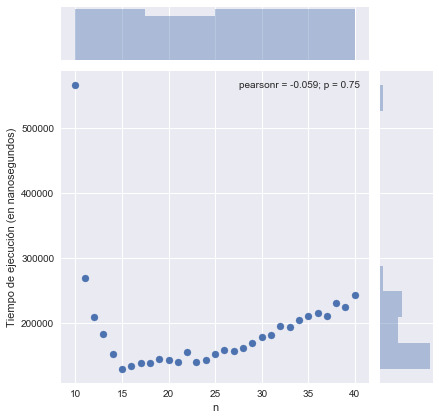
\includegraphics[scale=0.6]{img/exact-bad.png}
\end{minipage}
\hfill
\begin{minipage}{0.44\textwidth}
	\begin{center}
		Datos del gráfico

		\begin{tabular}{ | l |}
			\hline
			m = 40 \\
			\hline
		\end{tabular}
	\end{center}
\end{minipage}

Si bien nuestro análisis dio una cota de complejidad superior en base a $n$, no debemos descartar el hecho que un grafo con más nodos y misma cantidad de aristas puede poseer menos cliques. Por lo tanto, al generar cliques de mayor tamaño en base a otras más pequeñas, o al calcular la frontera de todas las cliques halladas, la cantidad de cliques a procesar puede ser mucho menor.

Por este motivo, decidimos analizar en particular el caso de los grafos completos. Allí podemos estudiar de manera determinística la cota propuesta:

\noindent
\begin{minipage}{0.49\textwidth}
	\hfill
	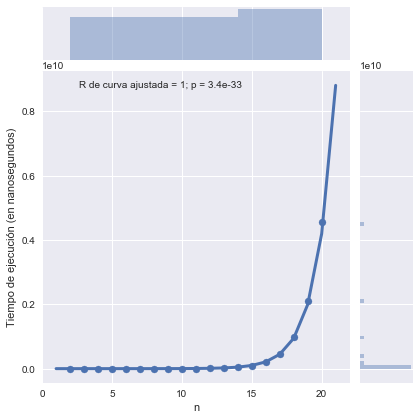
\includegraphics[scale=0.55]{img/exact-2n.png}
\end{minipage}
\hfill
\begin{minipage}{0.49\textwidth}
	\hfill
	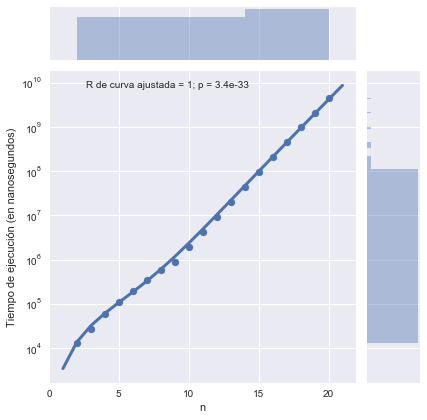
\includegraphics[scale=0.55]{img/exact-2n-log.png}
\end{minipage}

\begin{center}
	Datos de los gráficos

	\begin{tabular}{ | l l |}
		\hline
		\tikzcircle[fill=blue] & $f(x) = 200 * x * 2^x + 3000 * (x^2)$ \\
		\tikzcircle[fill=green] & $f(x) = 3000 * 2^x$ \\
		\hline
	\end{tabular}
\end{center}

Aqui podemos ver que el tiempo de ejecución se ajusta correctamente a la complejidad propuesta. A la derecha presentamos la misma gráfica en escala logarítmica, que nos permite apreciar la naturaleza exponencial del problema.
